\chapter{版图设计与验证}
本章节主要给出NORM指令基于第二章电路图的版图设计,包括电路图中的所有模块的版图设计,并对最终的设计进行DRC、LVS检查。
为了控制篇幅,这里仅给出所有子模块中几个主要模块的版图、DRC验证结果、LVS验证结果的截图。

{
\itshape
\bfseries
需要指出的是,在完成版图设计过程中,为了方便电源、地的走线,基本单元的高度被设置为同样的高度;为了减少需要的金属层,在连线过程中采取的基本原则是:横向采用M1层金属,纵向连线采用M2层金属,这样有利于减少不必要的绕线,因此,本次NORM的设计所有的连线都在M1、M2层内完成,没用到高层金属,但这样也导致设计中需要的M1、M2层间的通孔数量较多;最后,为了实现NORM指令最终的版图尽可能更规则,2路31位选择器采用双列的形式实现,这样就可以保证NORM模块最终可实现近似正方形的版图。
}

下面对几个主要模块进行说明,包括版图、DRC验证结果以及LVS验证结果。

\subsubsection{AND2模块}
本模块主要完成量输入与门的设计。其版图、DRC检查结果、LVS检查结果如图\ref{fig5.1}所示。
\begin{figure}[!hbtp]
\centering
\subfigure[AND2版图]{
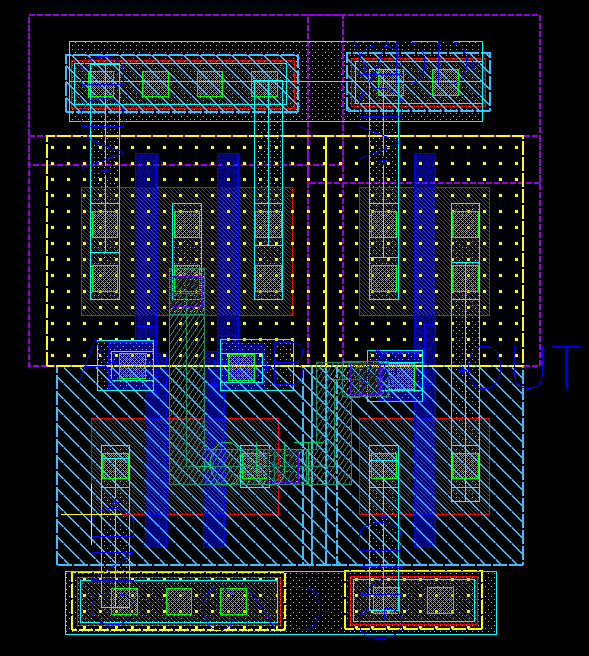
\includegraphics[width=0.7\textwidth]{chapter5/AND2}
\label{fig5.1a}
}
\subfigure[AND2 DRC验证结果]{
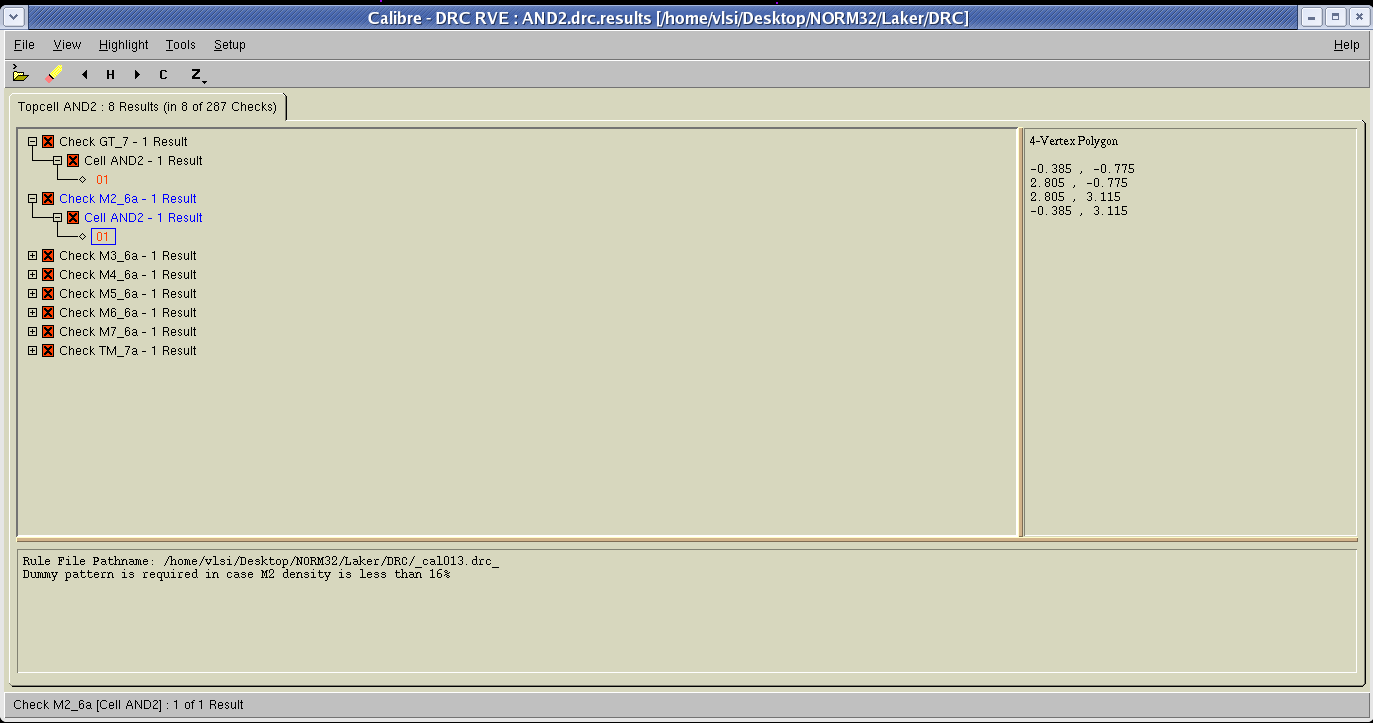
\includegraphics[width=0.7\textwidth]{chapter5/AND2_drc}
\label{fig5.1b}
}
\subfigure[AND2 LVS验证结果]{
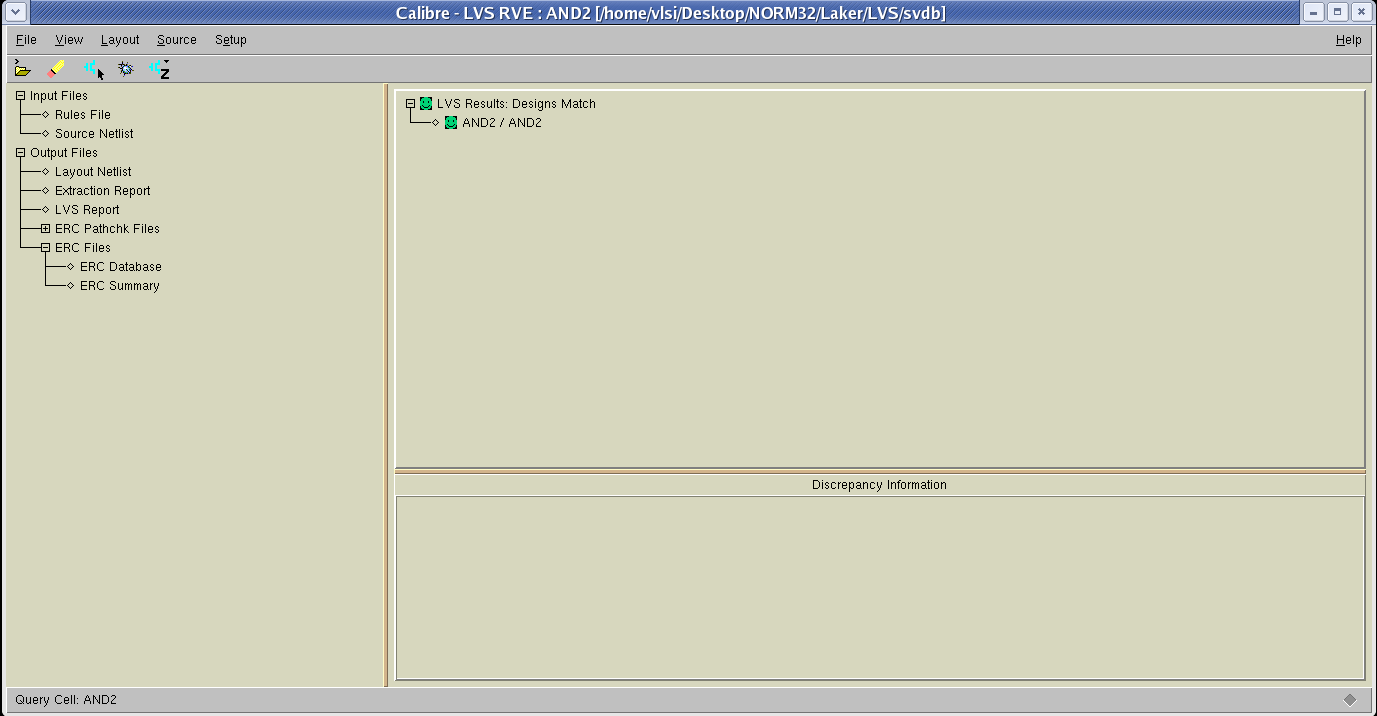
\includegraphics[width=0.7\textwidth]{chapter5/AND2_lvs}
\label{fig5.1c}
}
\caption{AND2版图设计及其验证结果}
\label{fig5.1}
\end{figure}
\subsubsection{IAO模块}
本模块主要完成三输入与或逻辑,即输入A与B,然后其结果再与C进行或操作。模块的版图等结果如图\ref{fig5.2}所示。
\begin{figure}[!hbtp]
\centering
\subfigure[IAO模块版图]{
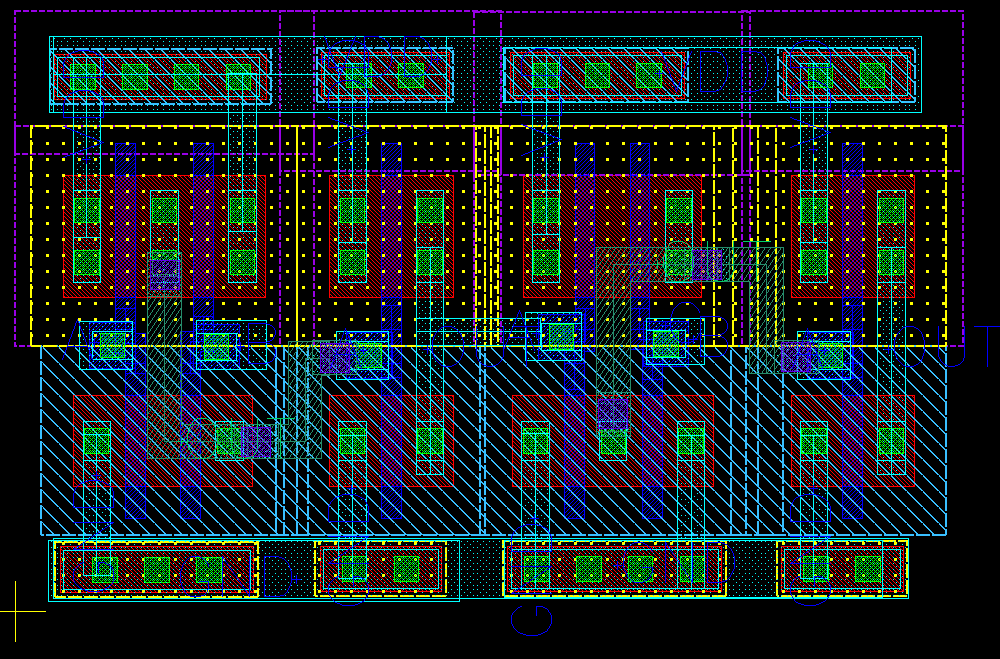
\includegraphics[width=0.7\textwidth]{chapter5/IAO}
\label{fig5.2a}
}
\subfigure[IAO DRC验证结果]{
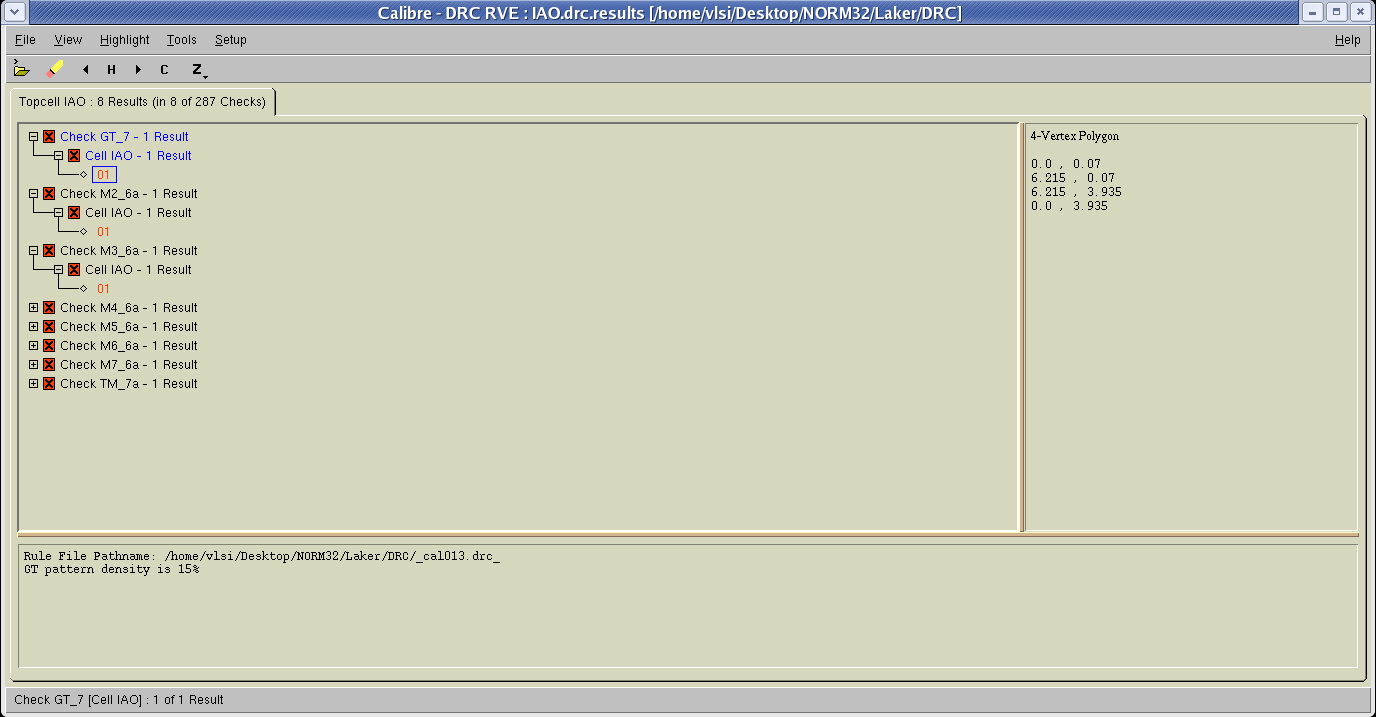
\includegraphics[width=0.7\textwidth]{chapter5/IAO_drc}
\label{fig5.2b}
}
\subfigure[IAO LVS验证结果]{
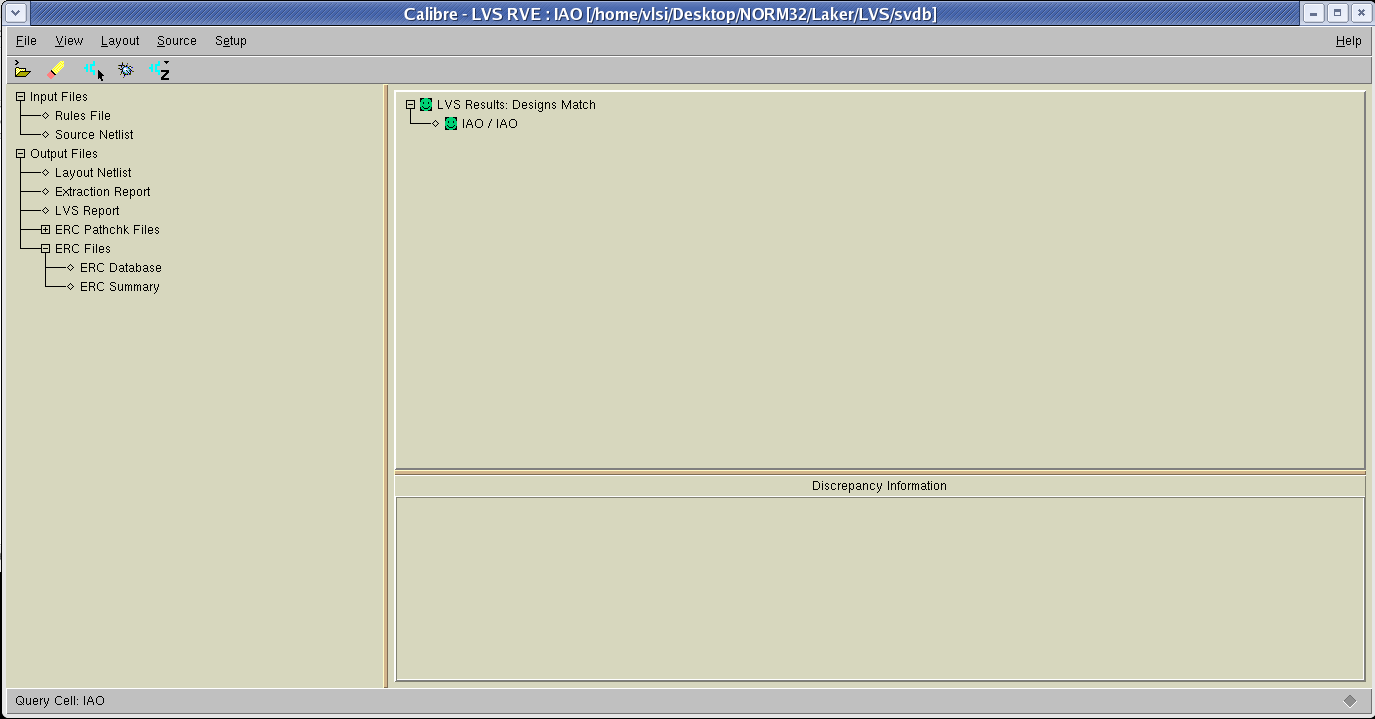
\includegraphics[width=0.7\textwidth]{chapter5/IAO_lvs}
\label{fig5.2c}
}
\caption{IAO版图设计及其验证结果}
\label{fig5.2}
\end{figure}
\subsubsection{MUX2\_1模块}
本模块主要完成两路一位选择器的功能,其结果如图\ref{fig5.3}所示,为防止出现有源区距离过小的DRC错误,其各个顶层单元之间的有源区彼此重合。
\begin{figure}[!hbtp]
\centering
\subfigure[MUX2\_1模块版图]{
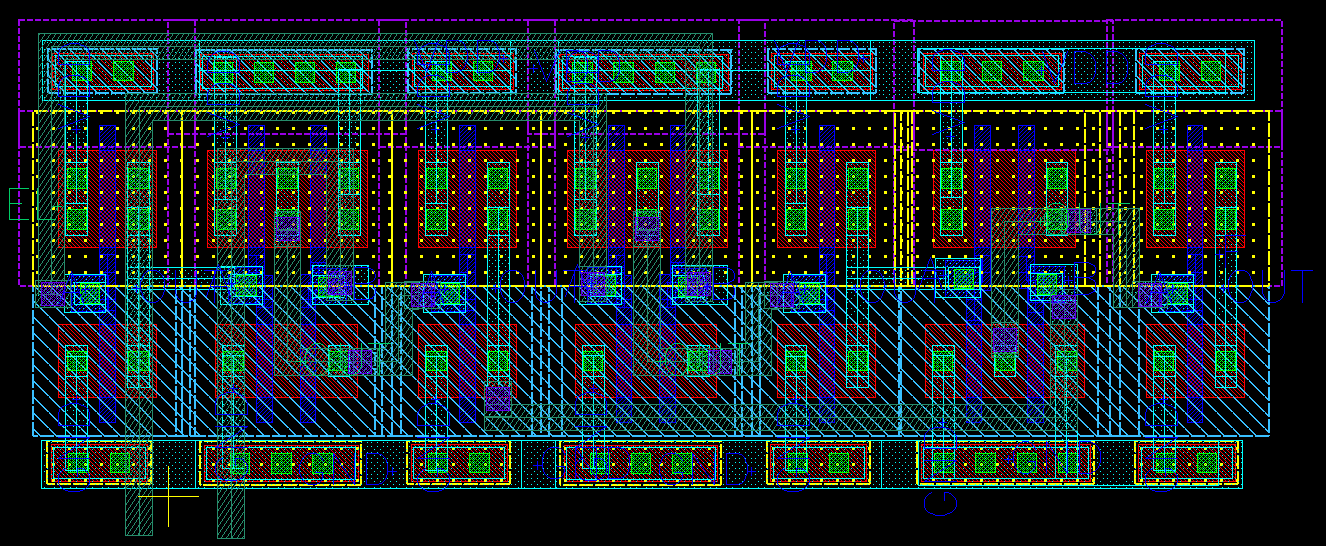
\includegraphics[width=0.7\textwidth]{chapter5/MUX2_1}
\label{fig5.3a}
}
\subfigure[MUX2\_1 DRC验证结果]{
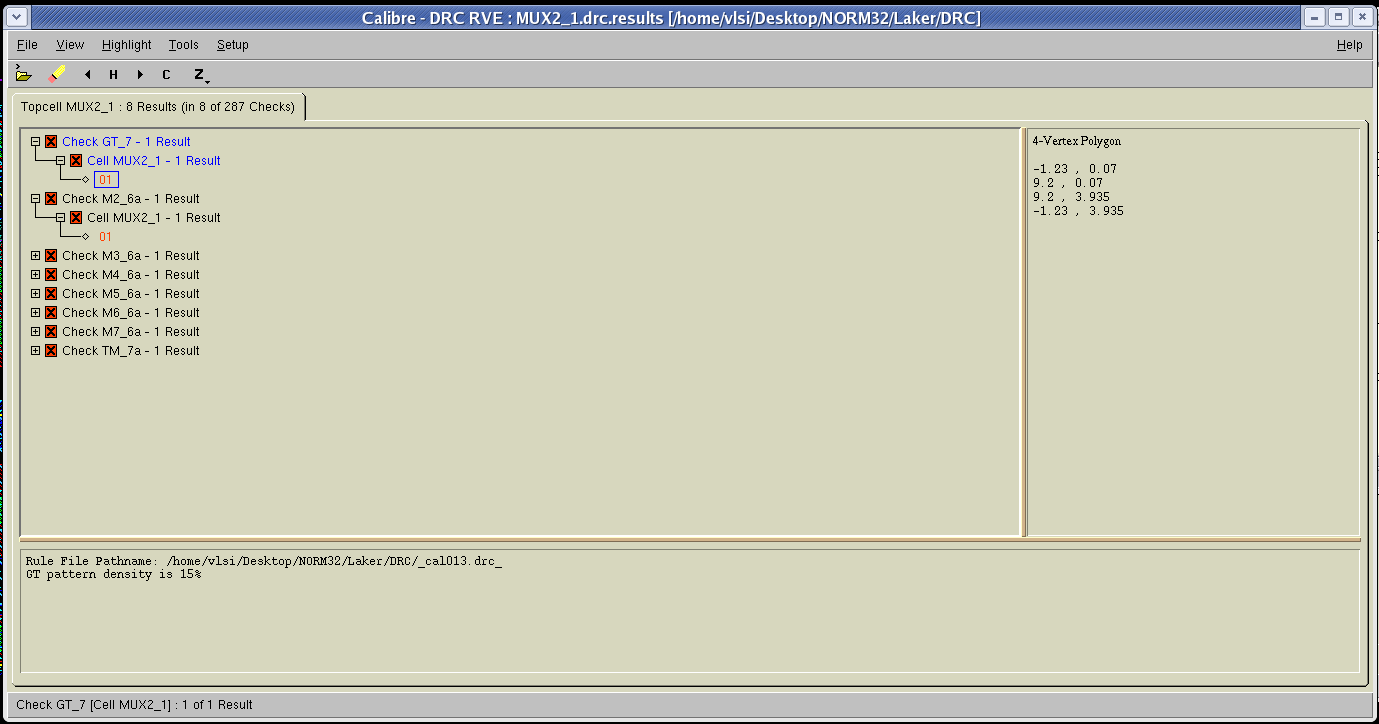
\includegraphics[width=0.7\textwidth]{chapter5/MUX2_1_drc}
\label{fig5.3b}
}
\subfigure[MUX2\_1 LVS验证结果]{
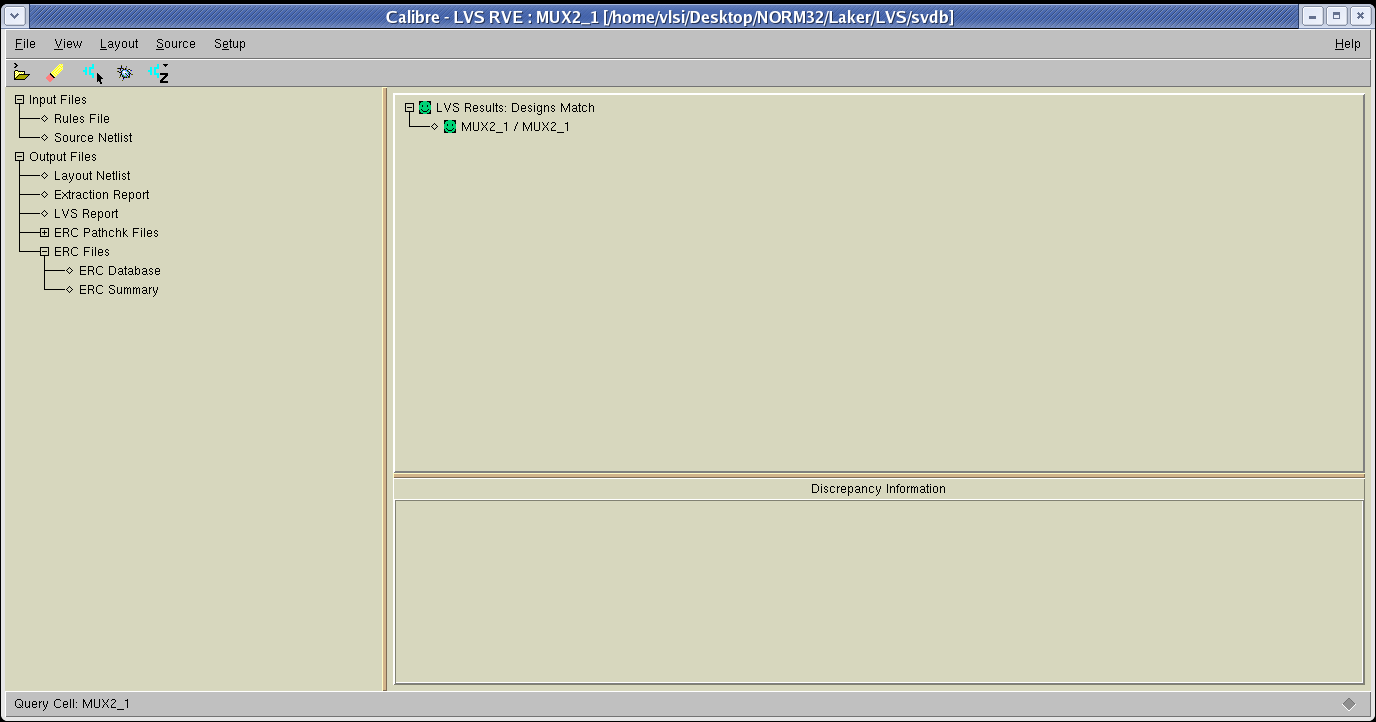
\includegraphics[width=0.7\textwidth]{chapter5/MUX2_1_lvs}
\label{fig5.3c}
}
\caption{MUX2\_1版图设计及其验证结果}
\label{fig5.3}
\end{figure}
\subsubsection{LZD4模块}
本模块完成4-bit输入数据的前导零检测功能,输出为2位,且真实结果为输出的反向。其结果如图\ref{fig5.4}所示。
\begin{figure}[!hbtp]
\centering
\subfigure[LZD4模块版图]{
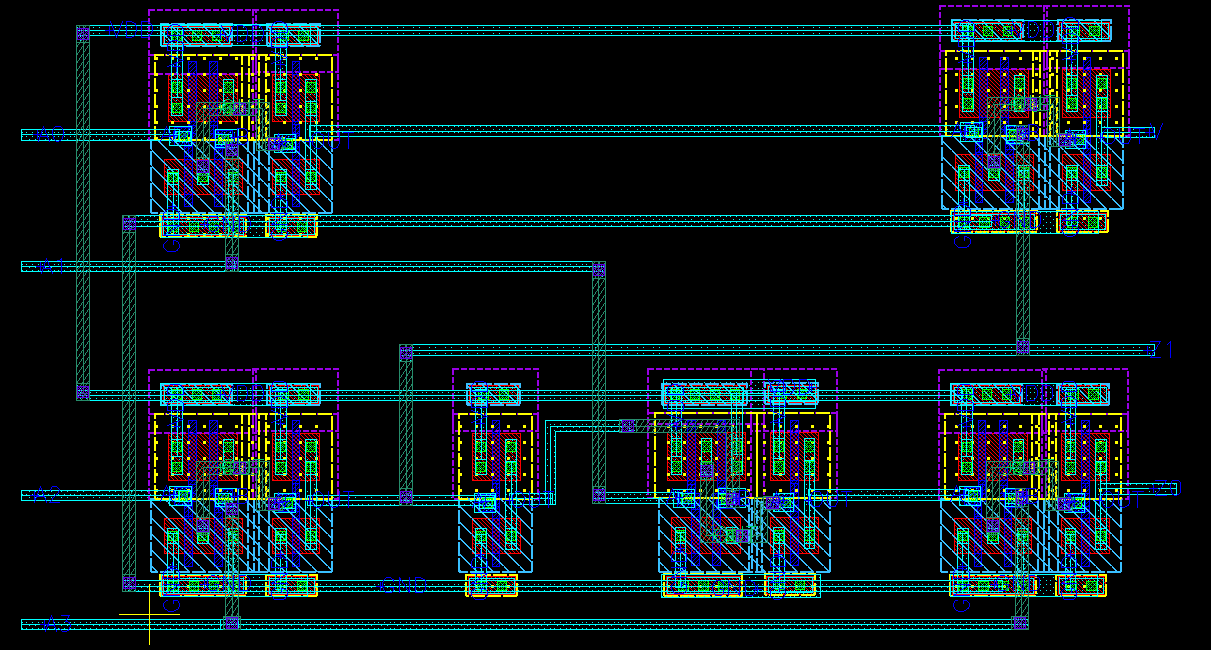
\includegraphics[width=0.7\textwidth]{chapter5/LZD4}
\label{fig5.4a}
}
\subfigure[LZD4 DRC验证结果]{
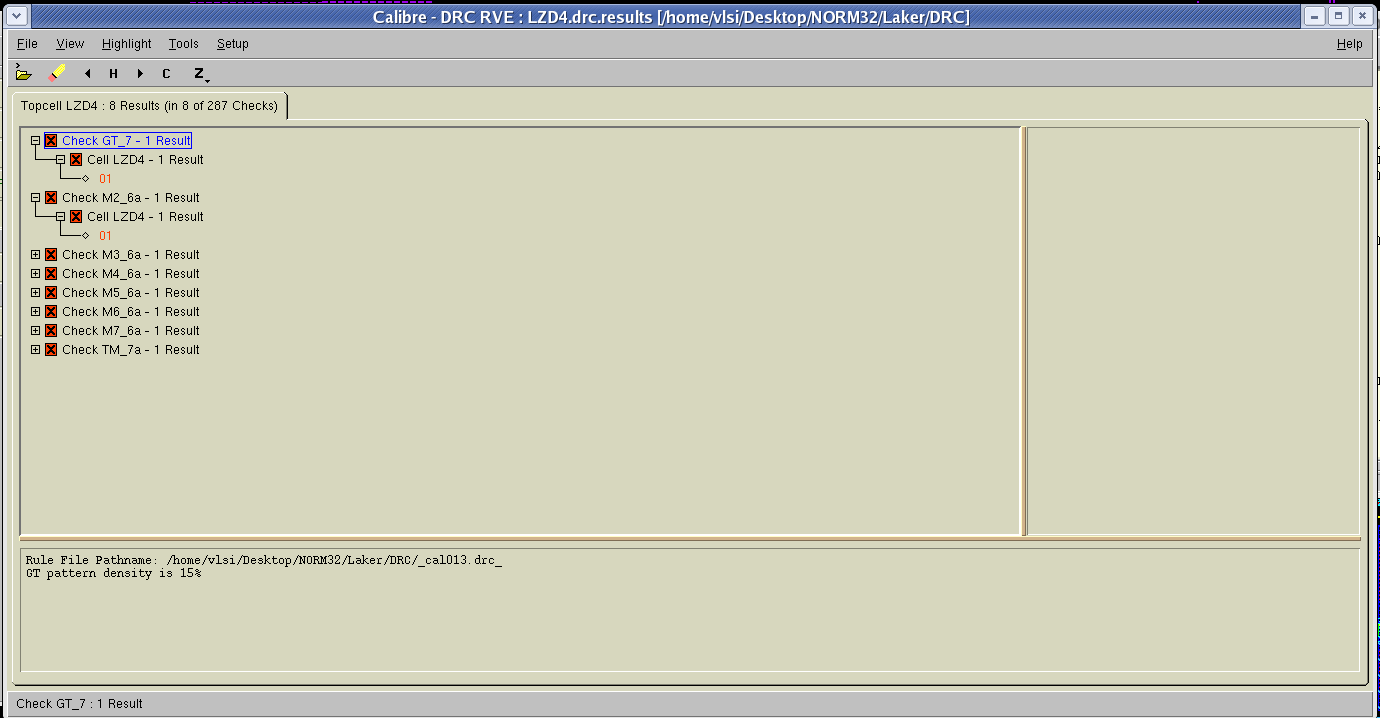
\includegraphics[width=0.7\textwidth]{chapter5/LZD4_drc}
\label{fig5.4b}
}
\subfigure[LZD4 LVS验证结果]{
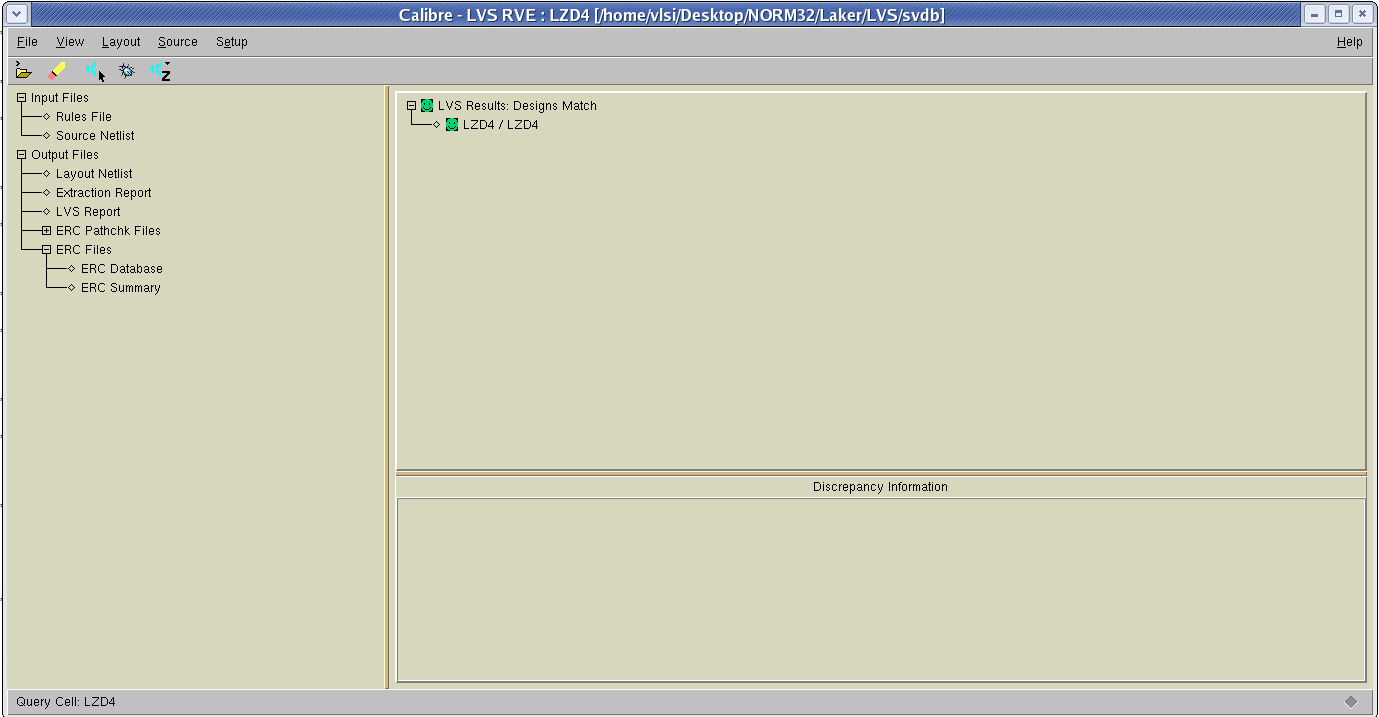
\includegraphics[width=0.7\textwidth]{chapter5/LZD4_lvs}
\label{fig5.4c}
}
\caption{LZD4版图设计及其验证结果}
\label{fig5.4}
\end{figure}
\subsubsection{LZD16模块}
本模块在LZD8(省略)的基础上完成16-bit输入数据的前导零计算功能,其输出同样为真实结果的反向,结果如图\ref{fig5.5}所示。
\begin{figure}[!hbtp]
\centering
\subfigure[LZD16模块版图]{
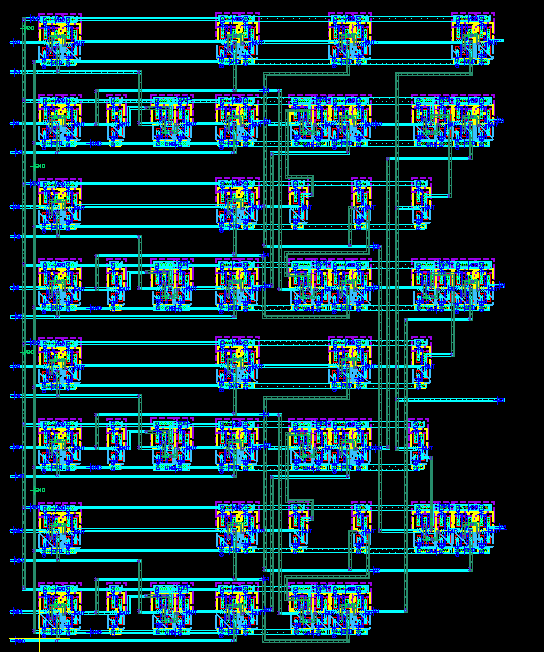
\includegraphics[width=0.7\textwidth]{chapter5/LZD16}
\label{fig5.5a}
}
\subfigure[LZD16 DRC验证结果]{
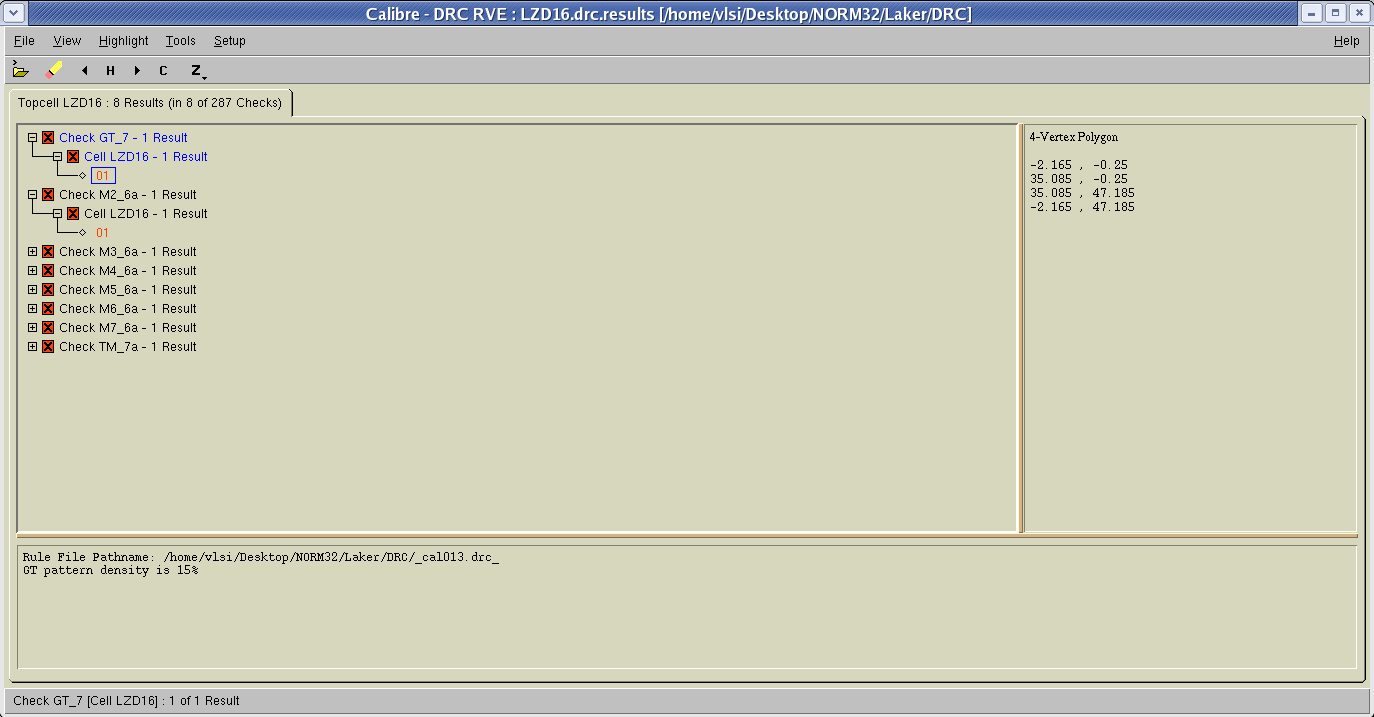
\includegraphics[width=0.7\textwidth]{chapter5/LZD16_drc}
\label{fig5.5b}
}
\subfigure[LZD16 LVS验证结果]{
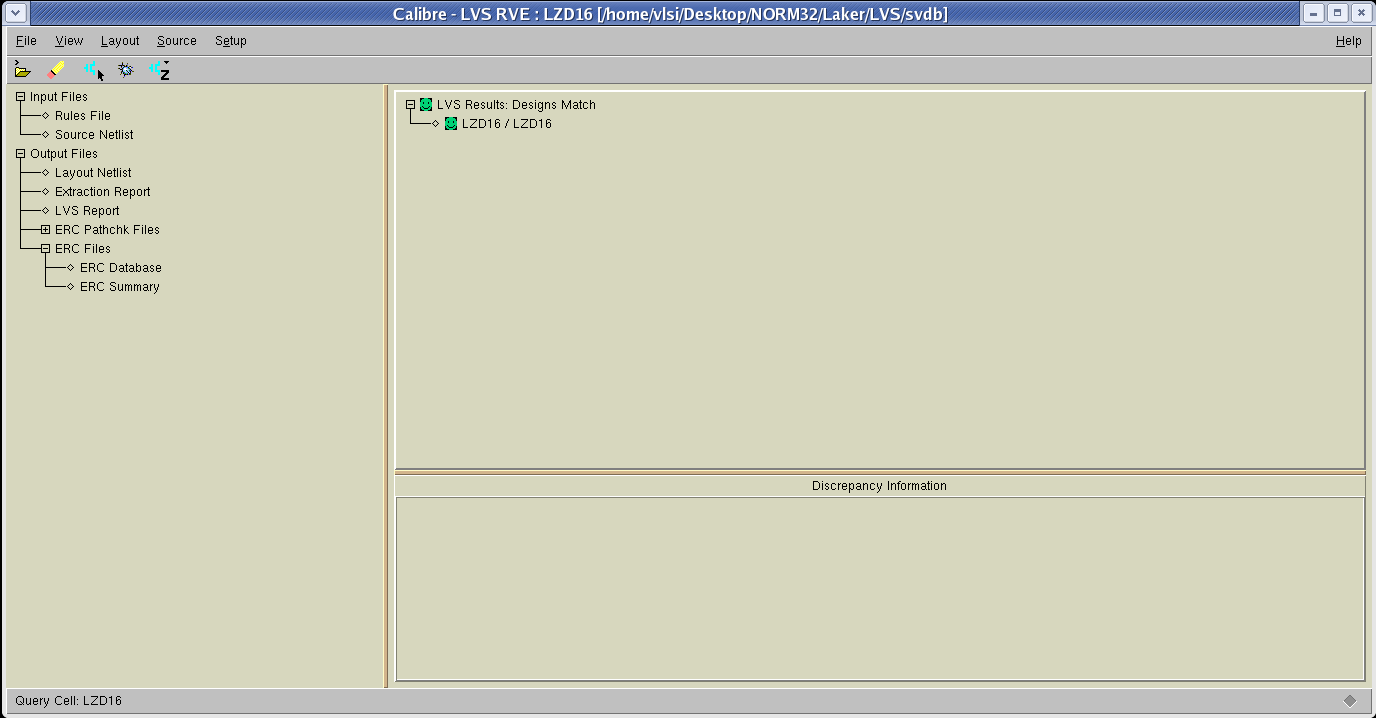
\includegraphics[width=0.7\textwidth]{chapter5/LZD16_lvs}
\label{fig5.5c}
}
\caption{LZD16版图设计及其验证结果}
\label{fig5.5}
\end{figure}

\subsubsection{LZDF模块}
本模块(LZDF: LZD Final)在LZD16的基础上完成32-bit输入数据的前导零计算功能,其输出同样为真实结果的反向,此外,其输入数据也由以前的直接输入变为从选择器输入,而两路选择器的输入,一路为未处理的输入数据,另一路为按位取反输入数据的结果,选择信号为输入数据的符号位。结果如图
\ref{fig5.6}所示。
\begin{figure}[!hbtp]
\centering
\subfigure[LZDF模块版图]{
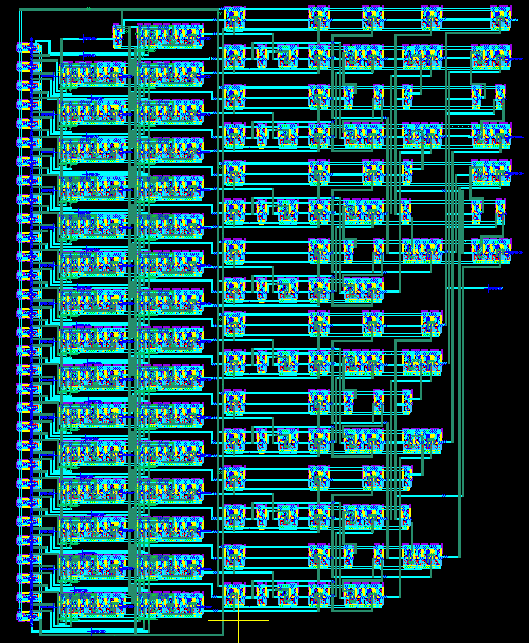
\includegraphics[width=0.6\textwidth]{chapter5/LZDF}
\label{fig5.6a}
}
\subfigure[LZDF DRC验证结果]{
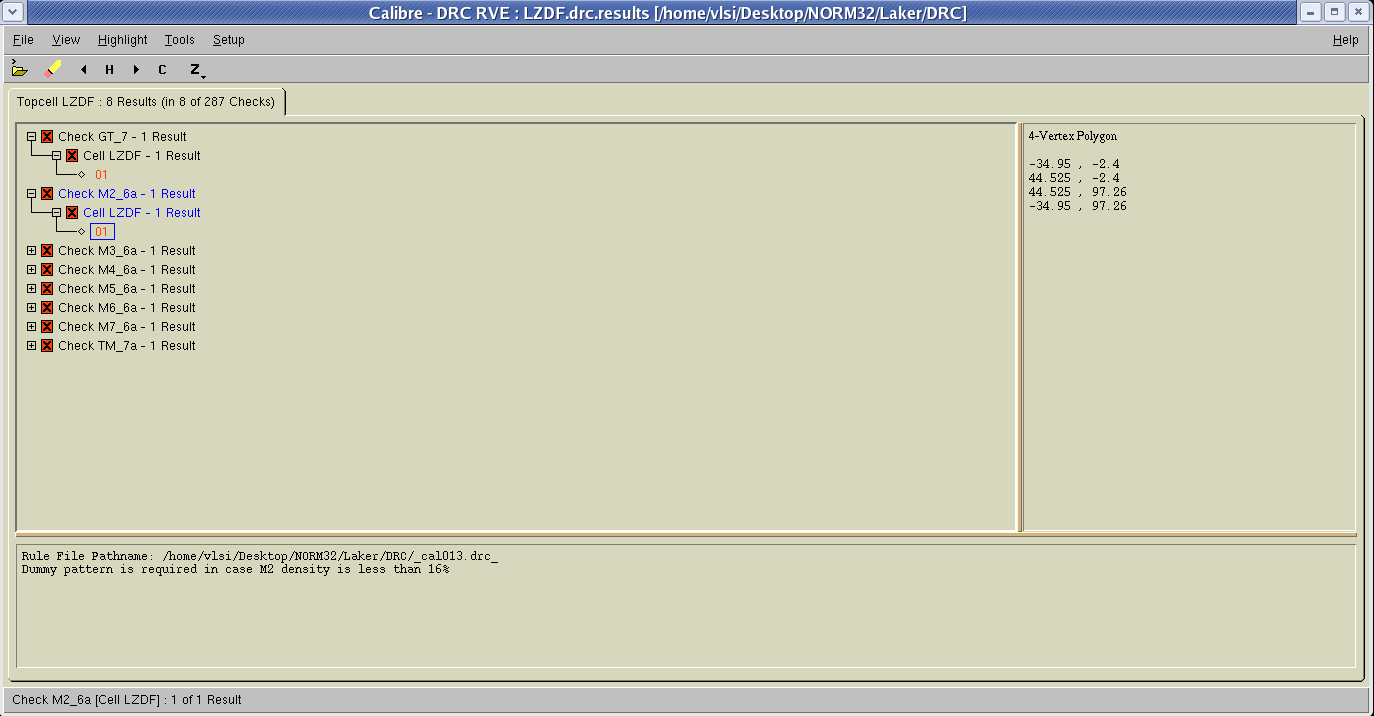
\includegraphics[width=0.7\textwidth]{chapter5/LZDF_drc}
\label{fig5.6b}
}
\subfigure[LZDF LVS验证结果]{
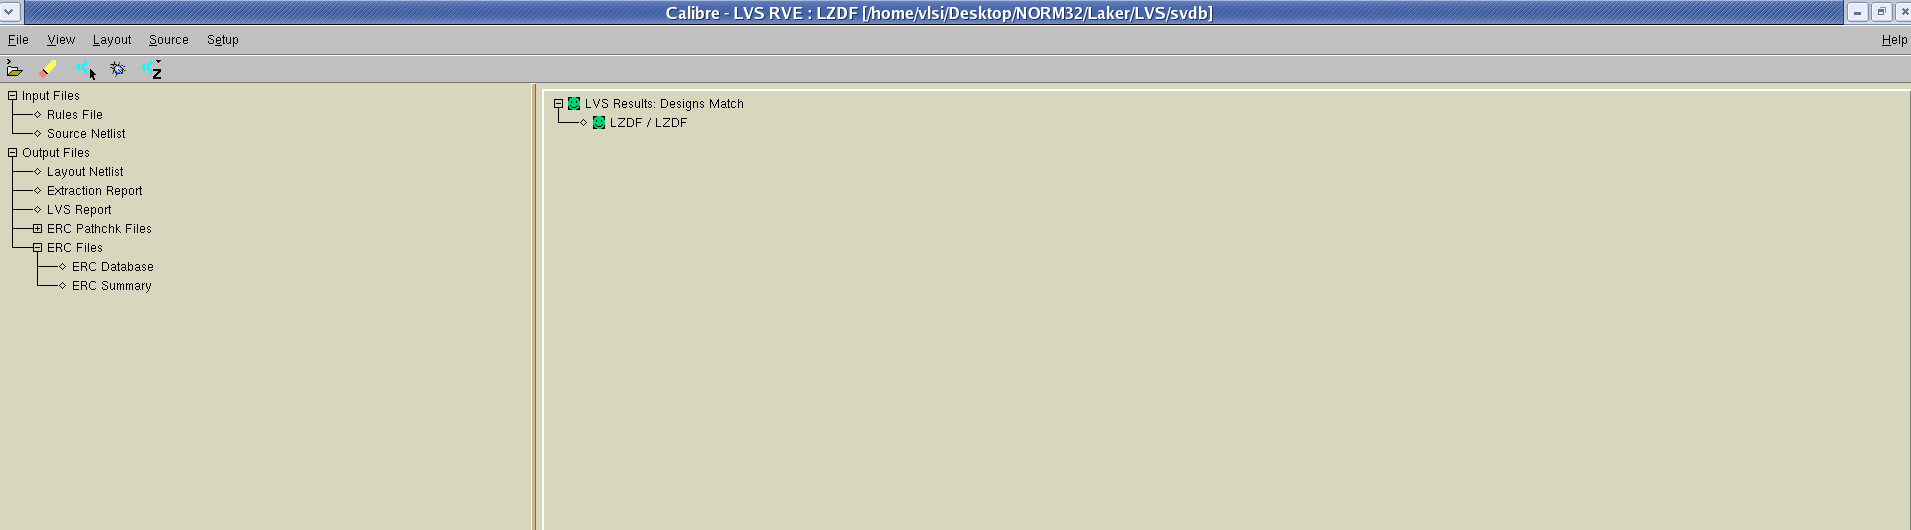
\includegraphics[width=0.7\textwidth]{chapter5/LZDF_lvs}
\label{fig5.6c}
}
\caption{LZDF版图设计及其验证结果}
\label{fig5.6}
\end{figure}
\subsubsection{NORM模块}
最后,本模块在LZDF模块的基础上,完成NORM指令模块的版图设计,其输出为32位,其中高位(31$\sim$5恒为0)。其结果如图\ref{fig5.7}所示。
\begin{figure}[!hbtp]
\centering
\subfigure[NORM模块版图]{
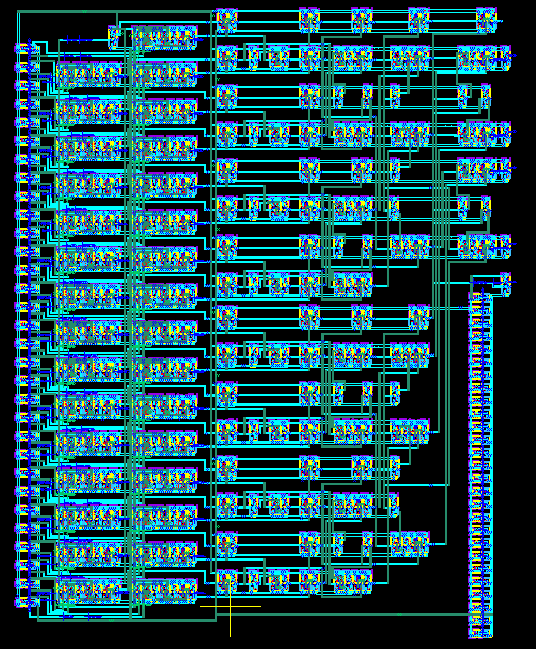
\includegraphics[width=0.7\textwidth]{chapter5/NORM}
\label{fig5.7a}
}
\subfigure[NORM DRC验证结果]{
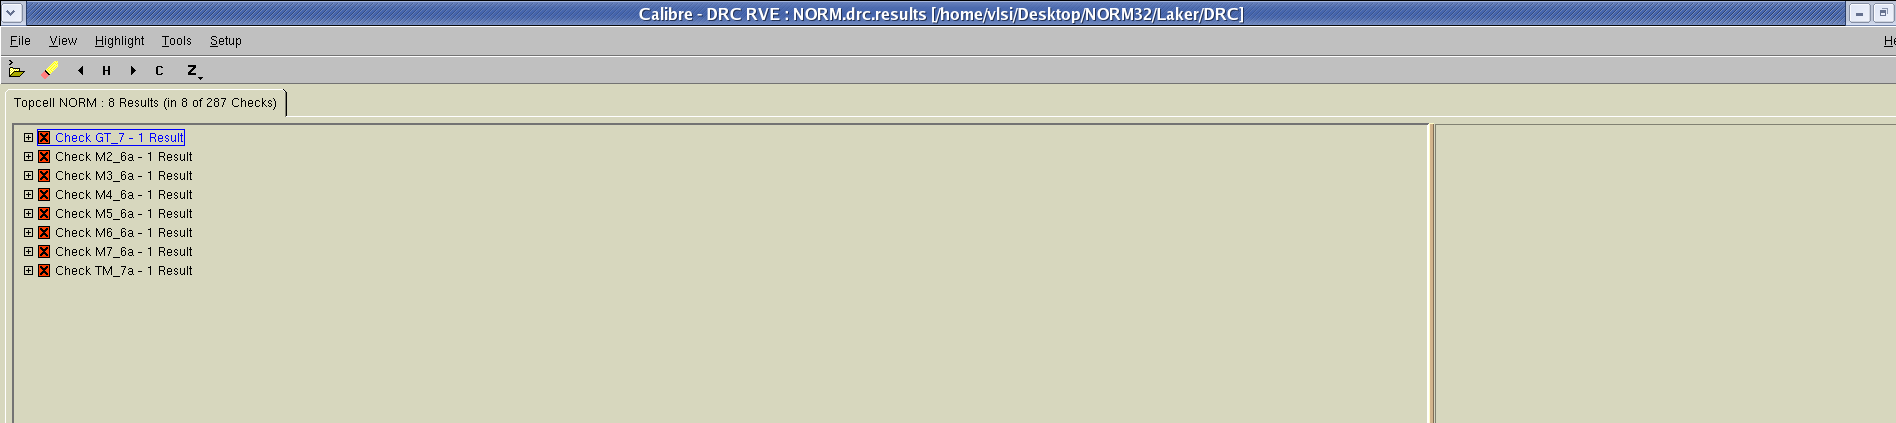
\includegraphics[width=0.7\textwidth]{chapter5/NORM_drc}
\label{fig5.7b}
}
\subfigure[NORM LVS验证结果]{
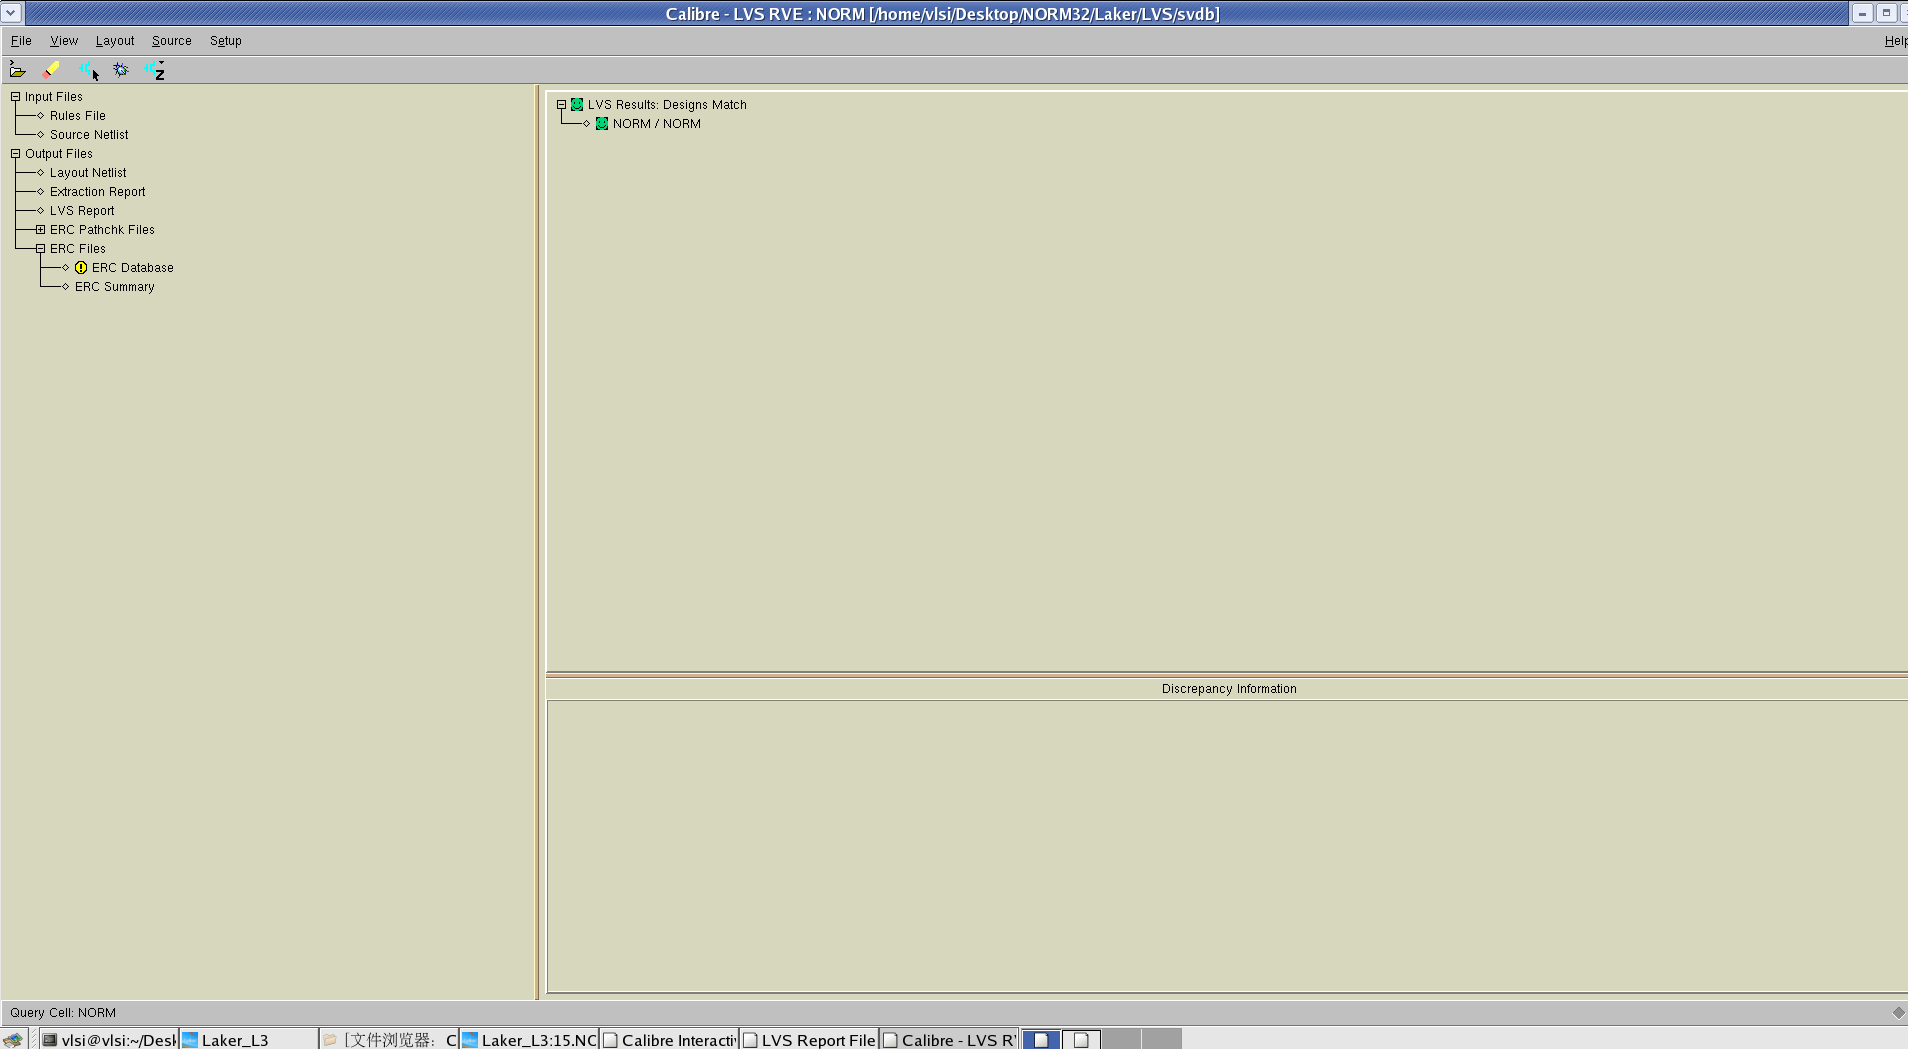
\includegraphics[width=0.7\textwidth]{chapter5/NORM_lvs}
\label{fig5.7c}
}
\caption{NORM 版图设计及其验证结果}
\label{fig5.7}
\end{figure}